\documentclass[10pt]{article}
\PassOptionsToPackage{numbers}{natbib}
\usepackage[preprint]{neurips_2026}
\usepackage{graphicx,booktabs,array,amsmath,amssymb,enumitem,microtype,hyperref}
\makeatletter\renewcommand{\@noticestring}{}\makeatother
\hypersetup{colorlinks=true,urlcolor=blue,citecolor=black,linkcolor=black}
\setlength{\parindent}{0pt}
\setlength{\parskip}{3pt}
\setlength{\textfloatsep}{7pt}
\setlength{\intextsep}{5pt}
\setlist{nosep,leftmargin=1.2em}
\title{What Post-training Rewards, and What It Misses}
\author{Advanced Topics in Machine Learning\\Fall 2026}

\begin{document}

\maketitle

\begin{abstract}
Post-training adjusts a language model after its initial training. It can raise a preference or reward score without making every answer more useful. This report compares three model-training methods (DPO, PPO, and GRPO) and two ways to score math answers: an exact answer checker and an AI judge. DPO modestly improves preference accuracy, but not the reward-model score. PPO's clipping setting would limit some token updates, but it did not affect the short policy runs. With GRPO, most prompts already produced different reward scores when each prompt had four sampled answers. Changing how answer length affects training changed token weights, but barely changed answer lengths. On GSM8K, neither RLVR nor RLAIF improved exact accuracy over SFT. The safety judge marked no safe answers as over-refusals, while a separate audit marked 44 of 120 reviewed safe-prompt answers that way. Code and saved results: \url{https://github.com/ttqureshi/ATML-PA2-LLM-PostTraining}.
\end{abstract}

\section{Introduction}
Language models first learn to predict text. Post-training then tries to make their answers more useful, preferred, or safe. Each training signal is only a stand-in for what we really want. A preference model may like a polished answer that contains a false claim. A checker that looks only at the final answer can miss faulty reasoning. A safety judge may treat a harmless question as dangerous.

This study asks three questions. When a training or judge score rises, do answers on separate test prompts also improve? How do update limits, group size, and answer-length rules affect training and responses? What errors appear when feedback comes from a learned preference model, an exact checker, or another language model?

\section{Experimental protocol}
All experiments use the course Qwen2.5-1.5B-Instruct models, the provided LoRA setup, the course data splits, and random seed 6304. DPO starts from the shared starting model. PPO and GRPO start from the provided halfway-trained models. A standard run makes 20 training updates. Unless noted, we test each model with the same prompts and text-generation settings. Task 4 tests four fixed models on 450 XSTest prompts. Task 5 uses 300 GSM8K questions, 100 SVAMP questions, and 80 pairs of deliberately changed answers based on 20 math problems.

\paragraph{Notation and model stages.} Pretraining teaches a model to predict the next word or token in text. Supervised fine-tuning (SFT) then trains it on example prompts and answers. Alignment further adjusts the SFT model using preferences or rewards. We use $x$ for a prompt and $y=(y_1,\ldots,y_T)$ for its answer, made of $T$ tokens. The policy $\pi_\theta$ is the model: it assigns probabilities to possible next tokens. The log-probability of a whole answer is the sum of the log-probabilities of its tokens: $\log\pi_\theta(y|x)=\sum_{t=1}^T\log\pi_\theta(y_t|x,y_{<t})$. The reference $\pi_{\rm ref}$ is the fixed starting model, usually the SFT model. A reward $r(x,y)$ is a number assigned to an answer; it is not the probability that the answer is correct. $\mathbb{E}$ means an average, and $\sigma(z)=1/(1+e^{-z})$ is the sigmoid function. We use $y^+$/$y^-$ for the preferred/rejected answers, $\beta$ for how strongly preferences are used, $\epsilon$ for PPO's update limit, and $\beta_{KL}$ for the penalty that keeps a model near its reference.

For preference feedback, a reward model $r_\psi(x,y)$ gives each answer a score. One way to turn two scores into a preference probability is $P(y^+\succ y^-|x)=\sigma(r_\psi(x,y^+)-r_\psi(x,y^-))$. The model is more likely to prefer the answer with the higher score. This score is still only a rough measure of answer quality.

\begin{table}[h]
\centering\small
\caption{What each comparison holds fixed and what it changes.}
\begin{tabular}{p{0.12\linewidth}p{0.36\linewidth}p{0.42\linewidth}}
\toprule
Task & Fixed evidence & Main change \\
\midrule
DPO & 300 held-out preference pairs; 246 length-stratified pairs & $\beta$ and length-balanced training pairs \\
PPO & Midpoint policy; 200 held-out prompts & Clipping $\epsilon$ and KL penalty $\beta_{KL}$ \\
GRPO & Midpoint policy; 200 held-out prompts & Group size and sequence normalization \\
Safety & 450 prompts per policy & SFT, standard DPO, PPO, and GRPO policies \\
Feedback & Same policy family; fixed math sets & Exact verifier versus AI preference reward \\
\bottomrule
\end{tabular}
\end{table}

\textbf{How to read the results.} Reward scores can be compared within one experiment, but they are not universal measures of quality. A sampled log-probability difference near zero is only an estimate; it does not prove that two models behave identically. We used one random seed and short training runs, so small differences are observations from these runs, not firm rankings that should generalize.

\section{Direct Preference Optimization}
DPO learns from pairs of answers: one marked preferred and the other rejected. It trains the model to make the preferred answer more likely than the rejected one, compared with the fixed reference model [1]. The main run used 1,500 pairs for one pass over the data (94 training steps). Each of the three shorter $\beta$ runs used 600 pairs (38 steps). On 300 separate test pairs, the main model chose the preferred answer 65.3\% of the time. Its reward score (1.164) was slightly below the reference model's (1.173). Their average answer lengths were nearly the same: 158 and 157 tokens.

For one preference triple $(x,y^+,y^-)$, define
\begin{equation}
z=\beta\{[\log\pi_\theta(y^+|x)-\log\pi_\theta(y^-|x)]-[\log\pi_{\rm ref}(y^+|x)-\log\pi_{\rm ref}(y^-|x)]\},\quad
\mathcal{L}_{\rm DPO}=-\mathbb{E}\log\sigma(z).\label{eq:dpo}
\end{equation}
The first bracket compares how likely the model finds the two answers. The second makes the same comparison for the reference model. So, if $z>0$, the updated model favors the preferred answer more than the reference did. Minimizing the loss encourages that change. $\beta$ controls its strength; it is not the learning rate.

\begin{table}[h]
\centering\scriptsize
\caption{DPO results. The standard run and short $\beta$ forks use different budgets.}
\begin{tabular}{lrrrrrr}
\toprule
Condition & Pairs/steps & Loss & Acc. & Sampled KL/token & Reward & Tokens (mean $\pm$ SD) \\
\midrule
Standard, $\beta=.10$ & 1500/94 & .674 & 65.3\% & $-0.000247$ & 1.164 & $158.0\pm105.5$ \\
Short, $\beta=.03$ & 600/38 & .691 & 65.0\% & $-0.000033$ & 1.183 & $156.4\pm105.7$ \\
Short, $\beta=.10$ & 600/38 & .686 & 63.3\% & $-0.000021$ & 1.192 & $156.8\pm105.9$ \\
Short, $\beta=.30$ & 600/38 & .678 & 63.7\% & $-0.000088$ & 1.175 & $156.3\pm105.8$ \\
\bottomrule
\end{tabular}
\end{table}

Across the short runs, test accuracy ranges from 63.3\% to 65.0\%. Neither reward nor the sampled log ratio steadily rises or falls as $\beta$ gets larger. So these runs do not show that stronger preference training reliably improves answers or moves the model farther from its starting point. The main run does better at choosing preferred answers on this test set, but its reward score moves in the opposite direction.

\begin{table}[h]
\centering\scriptsize
\caption{Length-controlled evaluation. Word-limit compliance is measured on only 10 prompts.}
\begin{tabular}{lrrrrrr}
\toprule
Training data & Overall acc. & Preferred longer & Matched & Rejected longer & Limit pass & Words (mean $\pm$ SD) \\
\midrule
Standard & 58.1\% & 42.7\% & 61.0\% & 70.7\% & 50\% & $53.0\pm34.0$ \\
Balanced & 62.6\% & 41.5\% & 64.6\% & 81.7\% & 60\% & $48.6\pm28.2$ \\
\bottomrule
\end{tabular}
\end{table}

Balancing answer lengths in the training pairs helps most when the rejected answer is longer: accuracy rises from 70.7\% to 81.7\%. It drops slightly when the preferred answer is longer. The balanced model also gives shorter answers on average and passes the word limit more often. But the word-limit check has only 10 prompts, too few to draw a strong conclusion. Figure~\ref{fig:dpo} shows these results.

\begin{figure}[h]
\centering
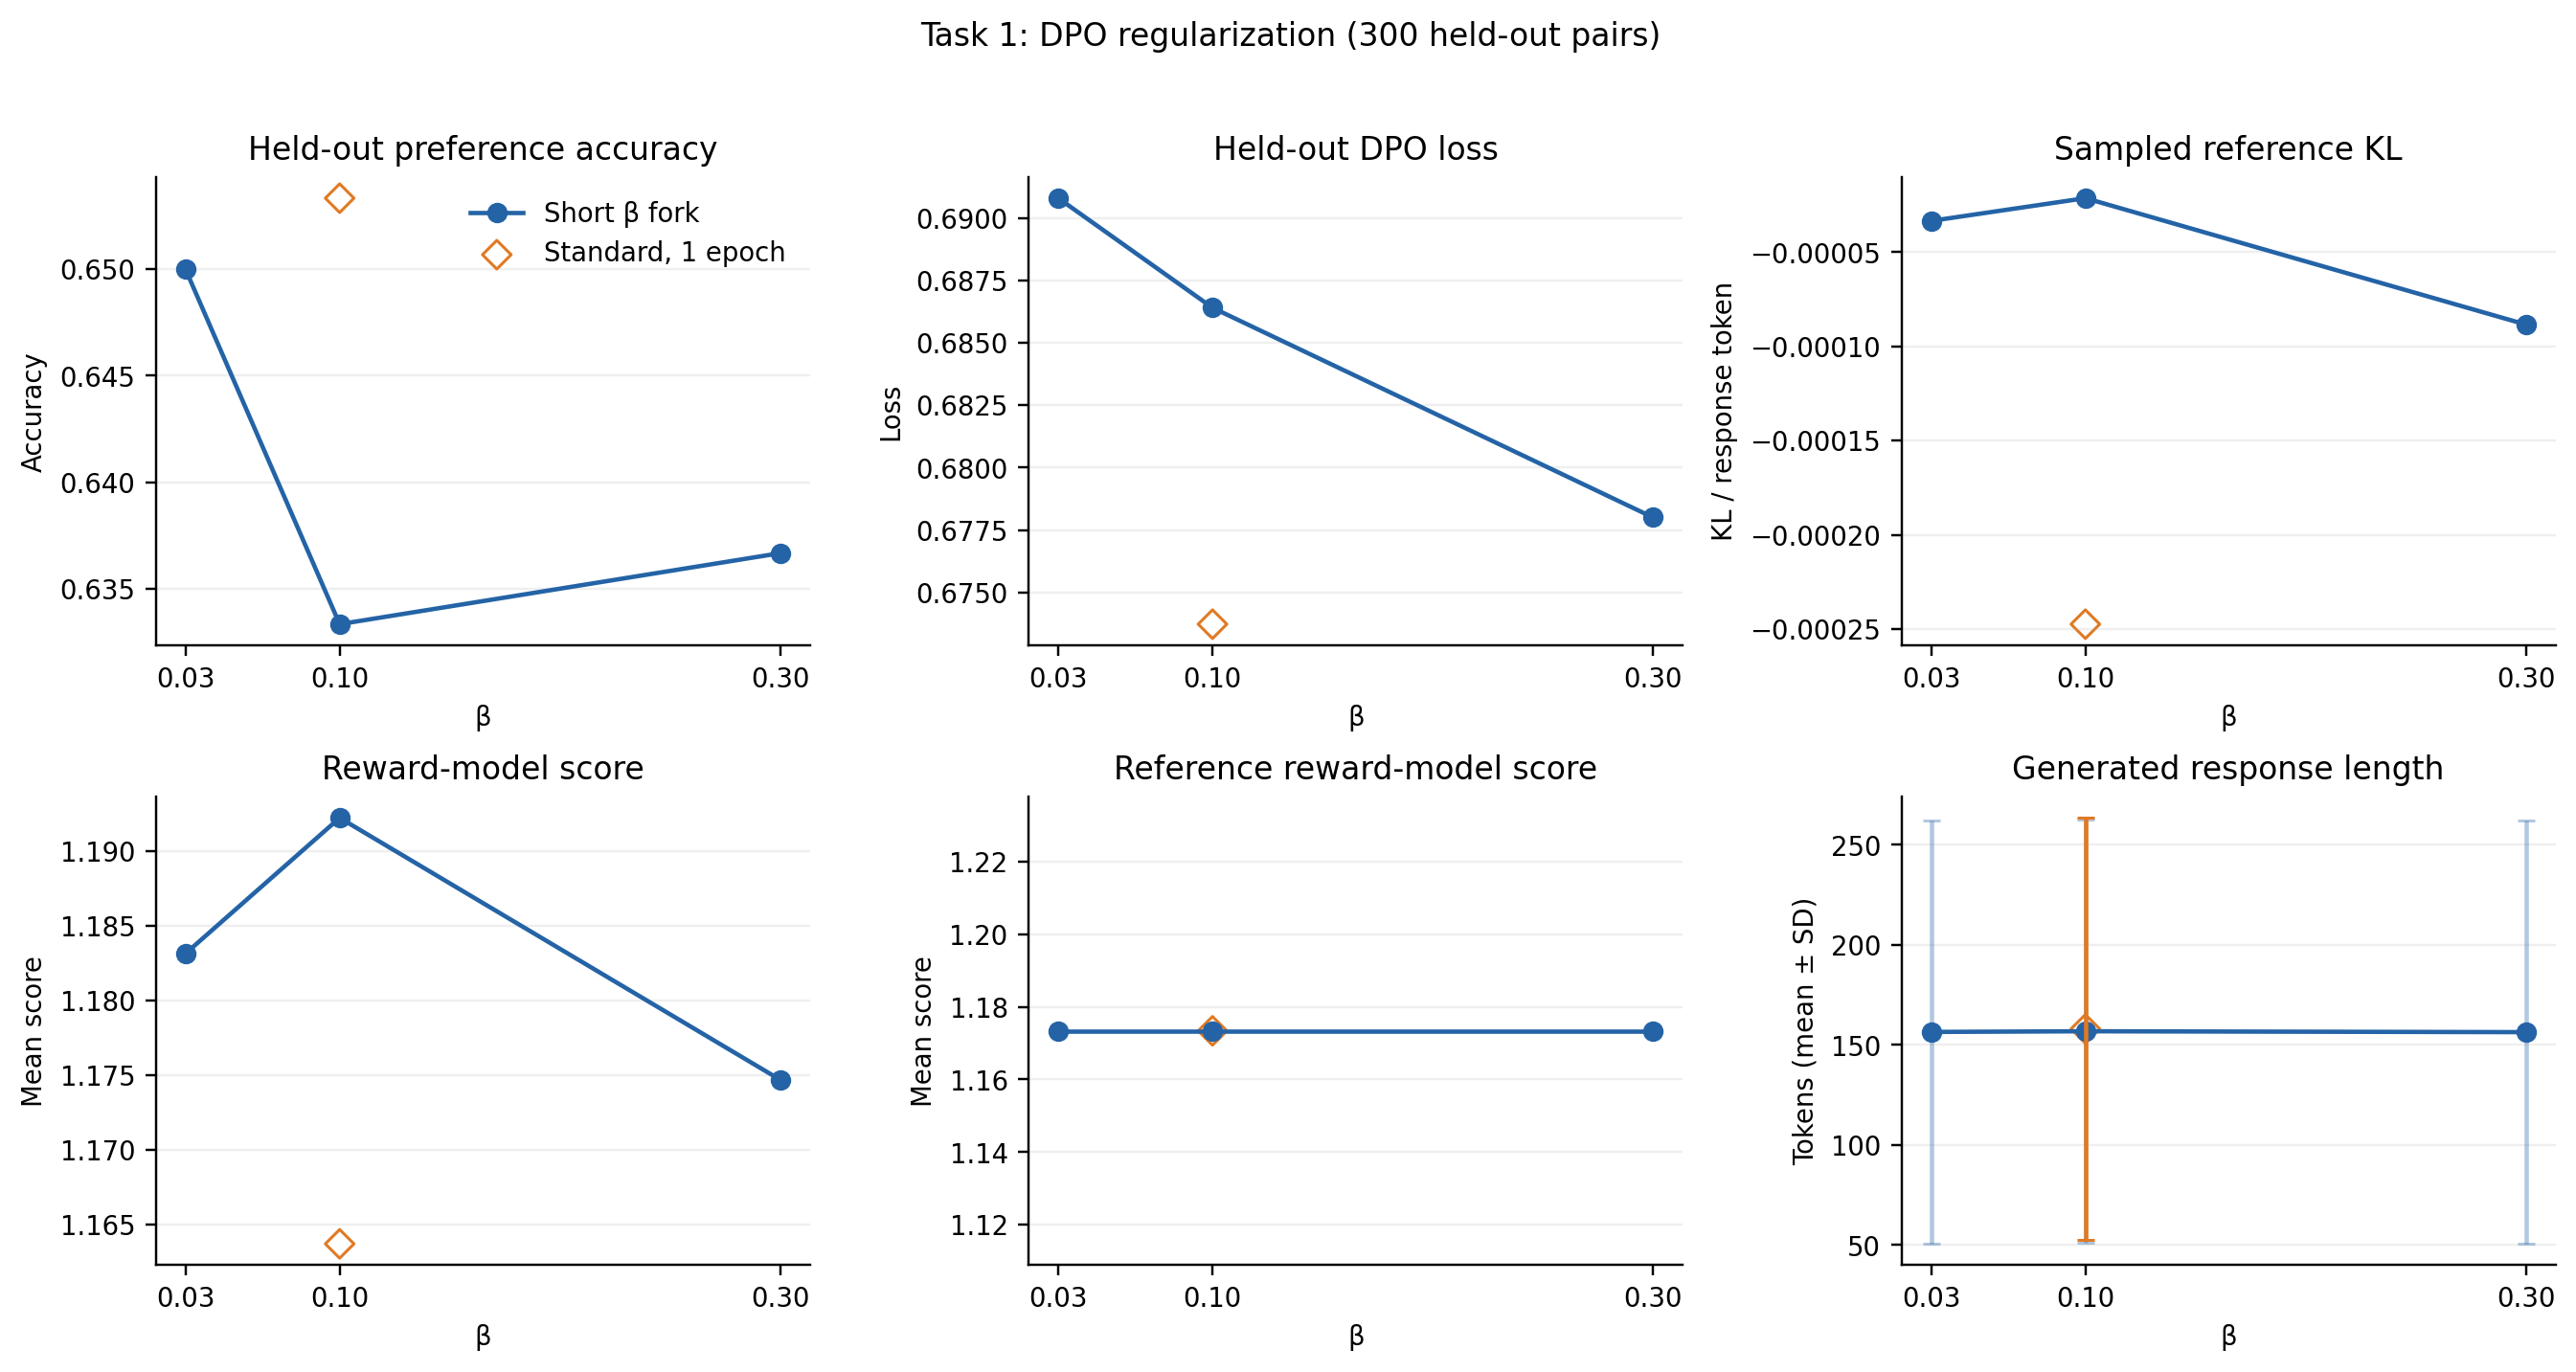
\includegraphics[width=.48\linewidth]{results/task1_dpo/figures/dpo_beta_tradeoffs.png}\hfill
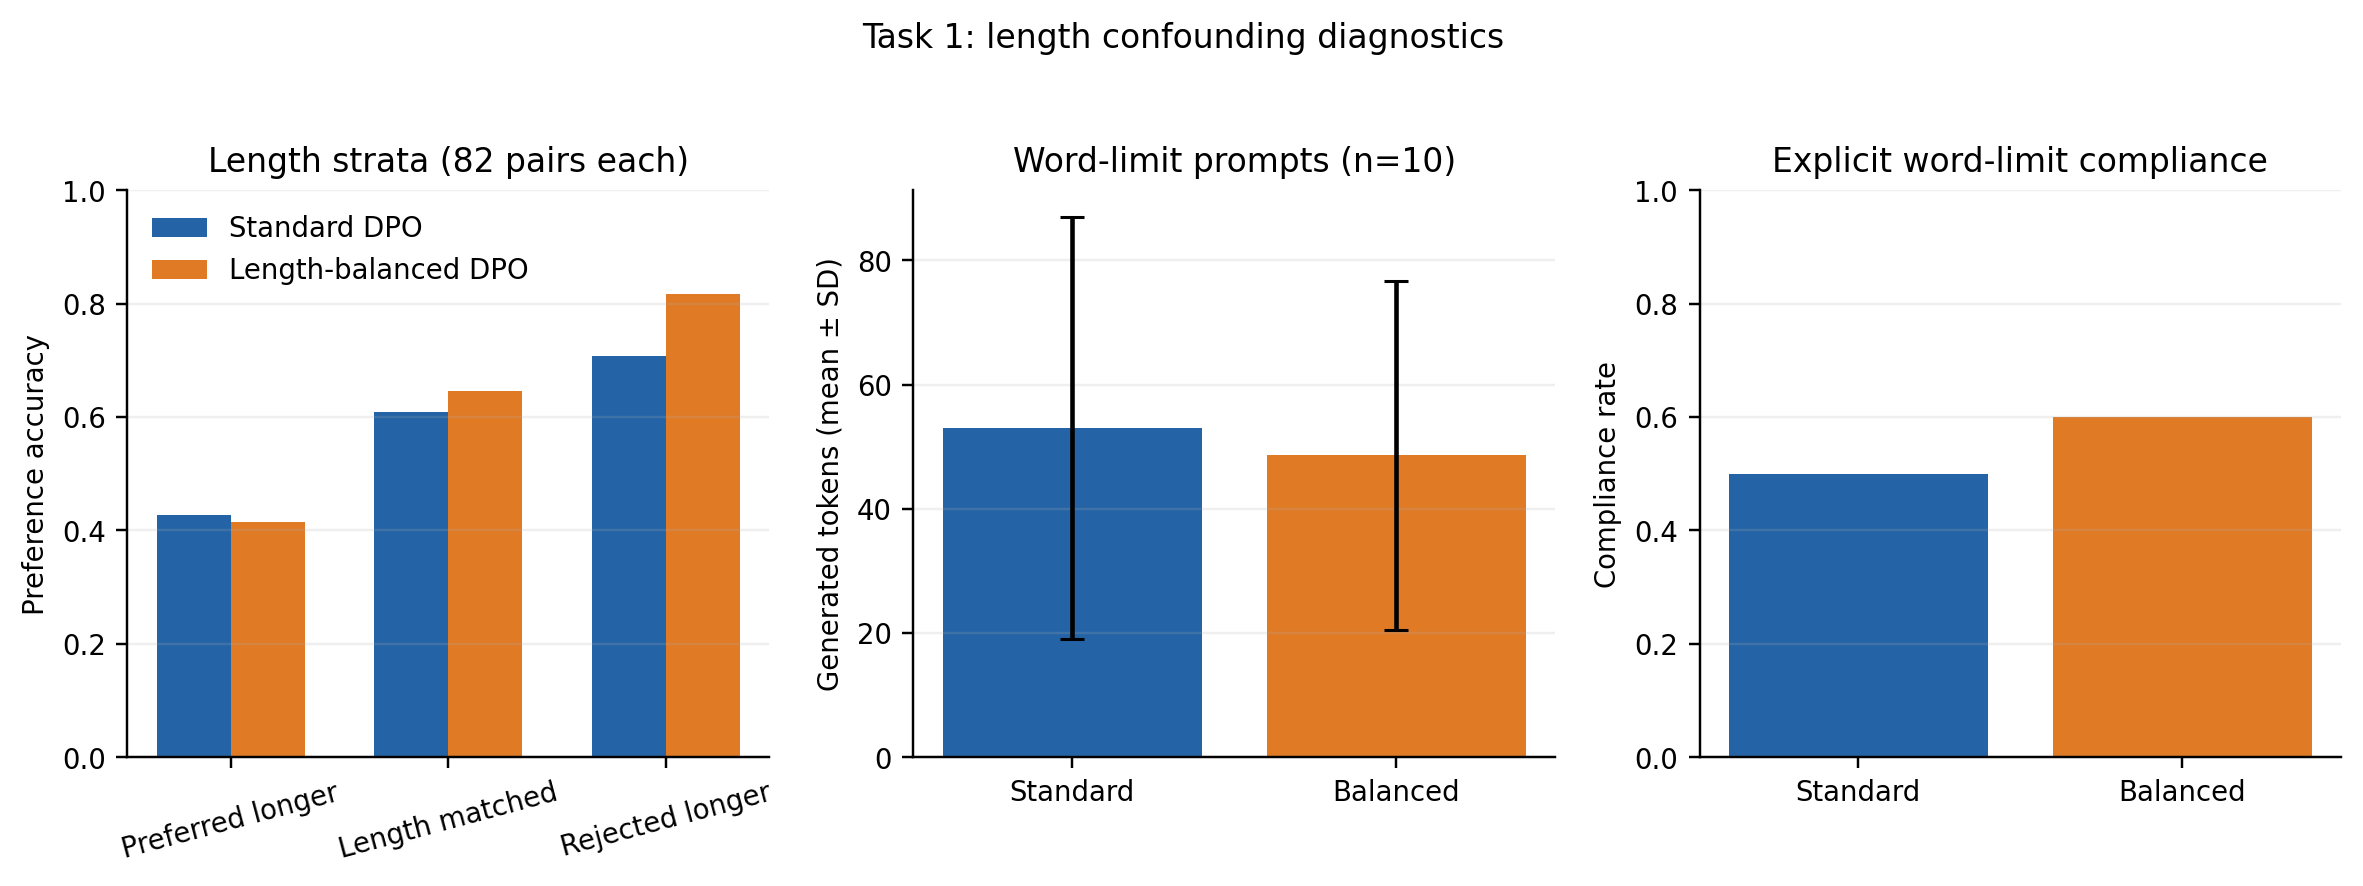
\includegraphics[width=.48\linewidth]{results/task1_dpo/figures/dpo_length_bias.png}
\caption{Left: preference scaling and measured outcomes. Right: preference accuracy across response-length strata.}
\label{fig:dpo}
\end{figure}

The SQL answer scored well, but it still did not do the requested job. Asked to select JSONB objects in an array by date, the model gives a score of 3.01, compared with 1.99 for the reference. The query does not correctly pull out the array elements or convert their dates, and the explanation describes an operator that the code does not use. The reward model can favor a confident-sounding answer without running the query. In another test, both models ignore a request to define overfitting in at most 25 words: each gives the same 30-word answer.

\section{Proximal Policy Optimization}
PPO trains on newly generated answers [2,3]. It limits how much a single update can change the model and adds a penalty for moving too far from the reference model. The main run made 20 updates, generated 5,202 tokens in 280 seconds, and used up to 8.37 GB of GPU memory. On 200 test prompts, its reward score was 1.482 and answers averaged 287 tokens (standard deviation 247). Entropy, a measure of how spread out the model's next-token choices are, was 1.020. The sampled KL estimate was $1.64\times10^{-5}$ per token. No training update reached the clipping limit.

At step $t$, the state $s_t=(x,y_{<t})$ contains the prompt and the answer tokens generated so far; the action $a_t=y_t$ is the next token. The old model $\pi_{\theta_{old}}$ generated the saved answer. The ratio $\rho_t=\exp(\log\pi_\theta(a_t|s_t)-\log\pi_{\theta_{old}}(a_t|s_t))$ compares how likely the new and old models are to produce that token. The advantage $A_t$ estimates whether the token led to a better result than expected. PPO maximizes
\begin{equation}
L_{clip}=\mathbb{E}_t\min\{\rho_t A_t,\operatorname{clip}(\rho_t,1-\epsilon,1+\epsilon)A_t\}.
\end{equation}
The clip operation keeps the ratio between $1-\epsilon$ and $1+\epsilon$. The minimum in the formula stops a large probability change from giving the update extra benefit. The critic $V_\phi(s)$ predicts the reward still to come from state $s$. We estimate the advantage using $\delta_t=r_t+\gamma V_\phi(s_{t+1})-V_\phi(s_t)$ and $A_t=\sum_{l=0}^{T-t-1}(\gamma\lambda)^l\delta_{t+l}$. Here $r_t$ is the reward at step $t$, $\gamma=1$ discounts future rewards, and $\lambda=.95$ controls how much the estimate relies on the critic; after the final token, the predicted future reward is zero. At each answer token, the reward also includes $-\beta_{KL}(\log\pi_{old}-\log\pi_{ref})$, which penalizes moving away from the reference. The task reward is added at the end of the answer. Entropy is recorded for monitoring, but this run does not train directly to increase it.

\begin{table}[h]
\centering\scriptsize
\caption{Cached clipping geometry and matched 8-update forks. Update clip fraction was zero in all three forks.}
\begin{tabular}{rrrrrr}
\toprule
$\epsilon$ & Cached clip frac. & Affected tokens & Held-out reward & KL/token & Length (mean $\pm$ SD) \\
\midrule
.05 & 15.4\% & 7.61\% & 1.528 & $6.01\times10^{-5}$ & $295.9\pm241.0$ \\
.20 & 4.13\% & 1.97\% & 1.528 & $6.01\times10^{-5}$ & $295.9\pm241.0$ \\
.50 & 2.11\% & 1.01\% & 1.528 & $6.01\times10^{-5}$ & $295.9\pm241.0$ \\
\bottomrule
\end{tabular}
\end{table}

The saved batch shows the expected pattern: a tighter limit clips more token ratios. But the short training runs did not learn different models. Their adapters and test outputs were identical, and no update reached the clipping limit. So this comparison shows how each setting would constrain the same saved batch; it does not show that one setting trained a better policy. Across the eight updates, the standard deviation of policy loss was 0.000209 and that of gradient norm was 0.765 for each fork. These short-run stability measures are identical because the forks produced the same updates.

\begin{table}[h]
\centering\scriptsize
\caption{KL-pressure forks (8 updates each; 200 held-out prompts).}
\begin{tabular}{rrrrr}
\toprule
$\beta_{KL}$ & Reward & KL/token & Entropy & Tokens (mean $\pm$ SD) \\
\midrule
0.00 & 1.464 & $9.20\times10^{-6}$ & 1.020 & $308.0\pm253.9$ \\
0.10 & 1.528 & $6.01\times10^{-5}$ & 1.034 & $295.9\pm241.0$ \\
0.20 & 1.443 & $2.31\times10^{-5}$ & 1.008 & $303.3\pm258.1$ \\
\bottomrule
\end{tabular}
\end{table}

The KL results do not move steadily with the penalty: the middle setting has the highest reward and KL estimate, and the largest penalty does not have the lowest KL. These small differences are not enough to rank the models. A high-reward answer about quantum mechanics is clear and relevant, but another high-reward answer gives an unchecked statistic about fast-food waste. A low-reward answer to a text adventure fails a simple request for five choices and gives only one incomplete question. The score catches that clear mistake, but it cannot check every fact in a polished answer.

\begin{figure}[h]
\centering
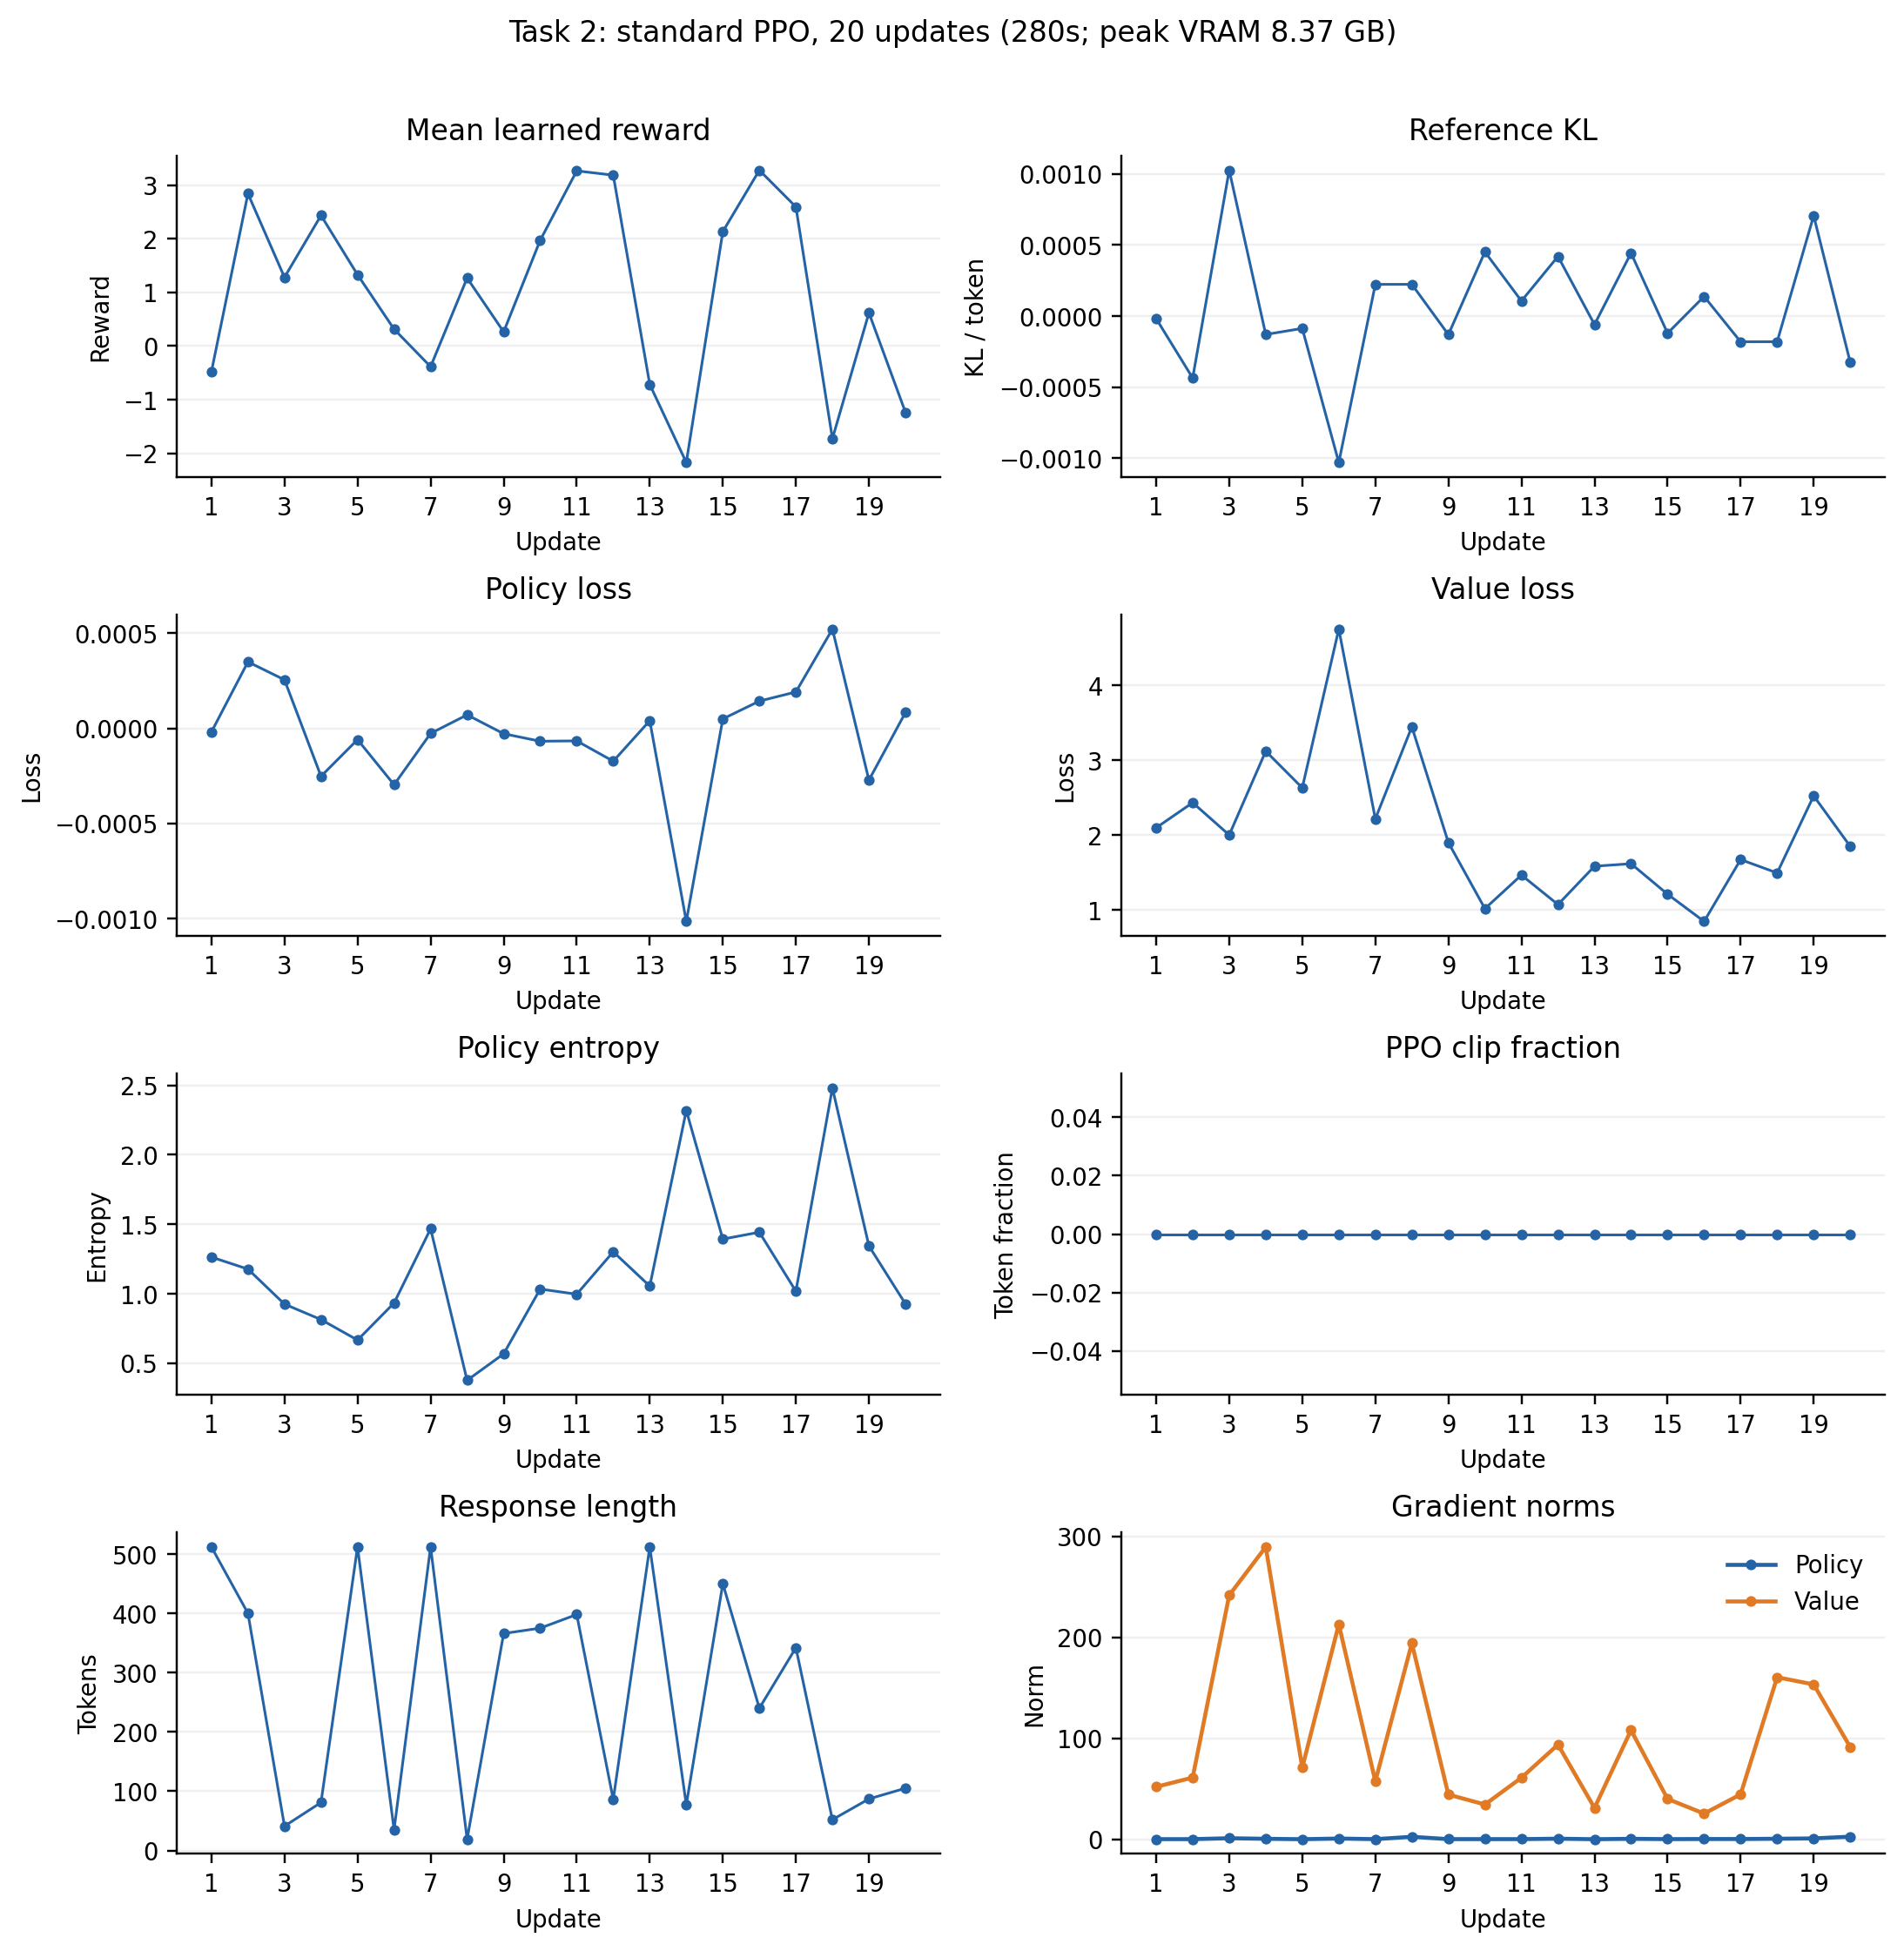
\includegraphics[width=.70\linewidth]{results/task2_ppo/figures/ppo_standard_trajectory.png}
\caption{Standard PPO training trajectory; the measured clipping fraction remains at zero.}
\end{figure}

\section{Group Relative Policy Optimization}
GRPO does not train PPO's separate value-prediction model. Instead, it compares several answers to the same prompt [4]. The main run used groups of four answers and made 20 updates. It generated 22,120 tokens (54\% of the configured maximum) in 398 seconds and used up to 5.82 GB of GPU memory. The average spread in scores within a group was 0.665; 5\% of groups gave every answer the same score. Mean entropy was 0.846, and training answers averaged 277 tokens. On 200 test prompts, the mean reward was 1.213, sampled KL was near zero, answers averaged 254 tokens, and 24\% reached the 512-token limit.

For prompt $x_b$, GRPO samples $K$ answers $y_{b,k}$ and gives each a score $r_{b,k}$. The group average score is $\mu_b=K^{-1}\sum_k r_{b,k}$. This implementation calculates each answer's advantage as $A_{b,k}=(r_{b,k}-\mu_b)/(\sigma_b+10^{-6})$, where $\sigma_b$ measures how much scores vary within the group. An answer above the group average has a positive advantage; one below it has a negative advantage. The token ratio $\rho_{b,k,t}=\pi_\theta(y_{b,k,t}|s)/\pi_{old}(y_{b,k,t}|s)$ compares the new and old models' probability for token $t$. $T_{b,k}$ is the answer length. The training loss is
\begin{equation}
\mathcal{L}_{GRPO}=-\frac{1}{BK}\sum_{b,k}\frac{1}{T_{b,k}}\sum_t\min\{\rho A,\operatorname{clip}(\rho,1-\epsilon,1+\epsilon)A\}+\beta_{KL}D(\pi_\theta,\pi_{ref}).
\end{equation}
Here $B$ is the number of prompts and $D$ is the penalty for moving away from the reference model. In this implementation, each token's penalty is estimated as $d=\exp(q)-q-1$, where $q=\log\pi_{ref}(y_t|s_t)-\log\pi_\theta(y_t|s_t)$; these token penalties are averaged over the answer. The lecture notes define the group advantage without dividing by $\sigma_b$; our code does divide by it. In canonical GRPO, each answer's token contributions are divided by that answer's length $T_{b,k}$. Dr. GRPO instead divides by the same maximum length for all answers. This changes how strongly short and long answers affect training [5].

\begin{table}[h]
\centering\scriptsize
\caption{Group-size study with a fixed budget of 192 generations. Prompts are ranked by mean reward over eight fixed completions; the lower half is hard and the upper half easy, with ties broken by source index.}
\begin{tabular}{rrrrrrrr}
\toprule
$K$ & Groups & Info. & Reward SD & Signal var. & Hard info. & Easy info. & Hard SD \\
\midrule
2 & 96 & 93.8\% & .385 & .937 & 89.6\% & 97.9\% & .528 \\
4 & 48 & 95.8\% & .541 & .958 & 91.7\% & 100\% & .712 \\
8 & 24 & 95.8\% & .619 & .958 & 91.7\% & 100\% & .800 \\
\bottomrule
\end{tabular}
\end{table}

Going from two answers per prompt to four makes it a little more likely that the answers get different scores. Going from four to eight does not improve that rate in this test, and it means testing half as many prompts with the same total of 192 answers. Easy prompts already produce useful score differences; the change is small on harder prompts. With this fixed budget, groups larger than four add little.

Removing the critic does not remove randomness. GRPO's training signal depends on which answers happen to be sampled. If every answer gets the same score, the group gives the model no direction for learning. More samples help only if they produce answers with different scores.

\begin{figure}[t]
\centering
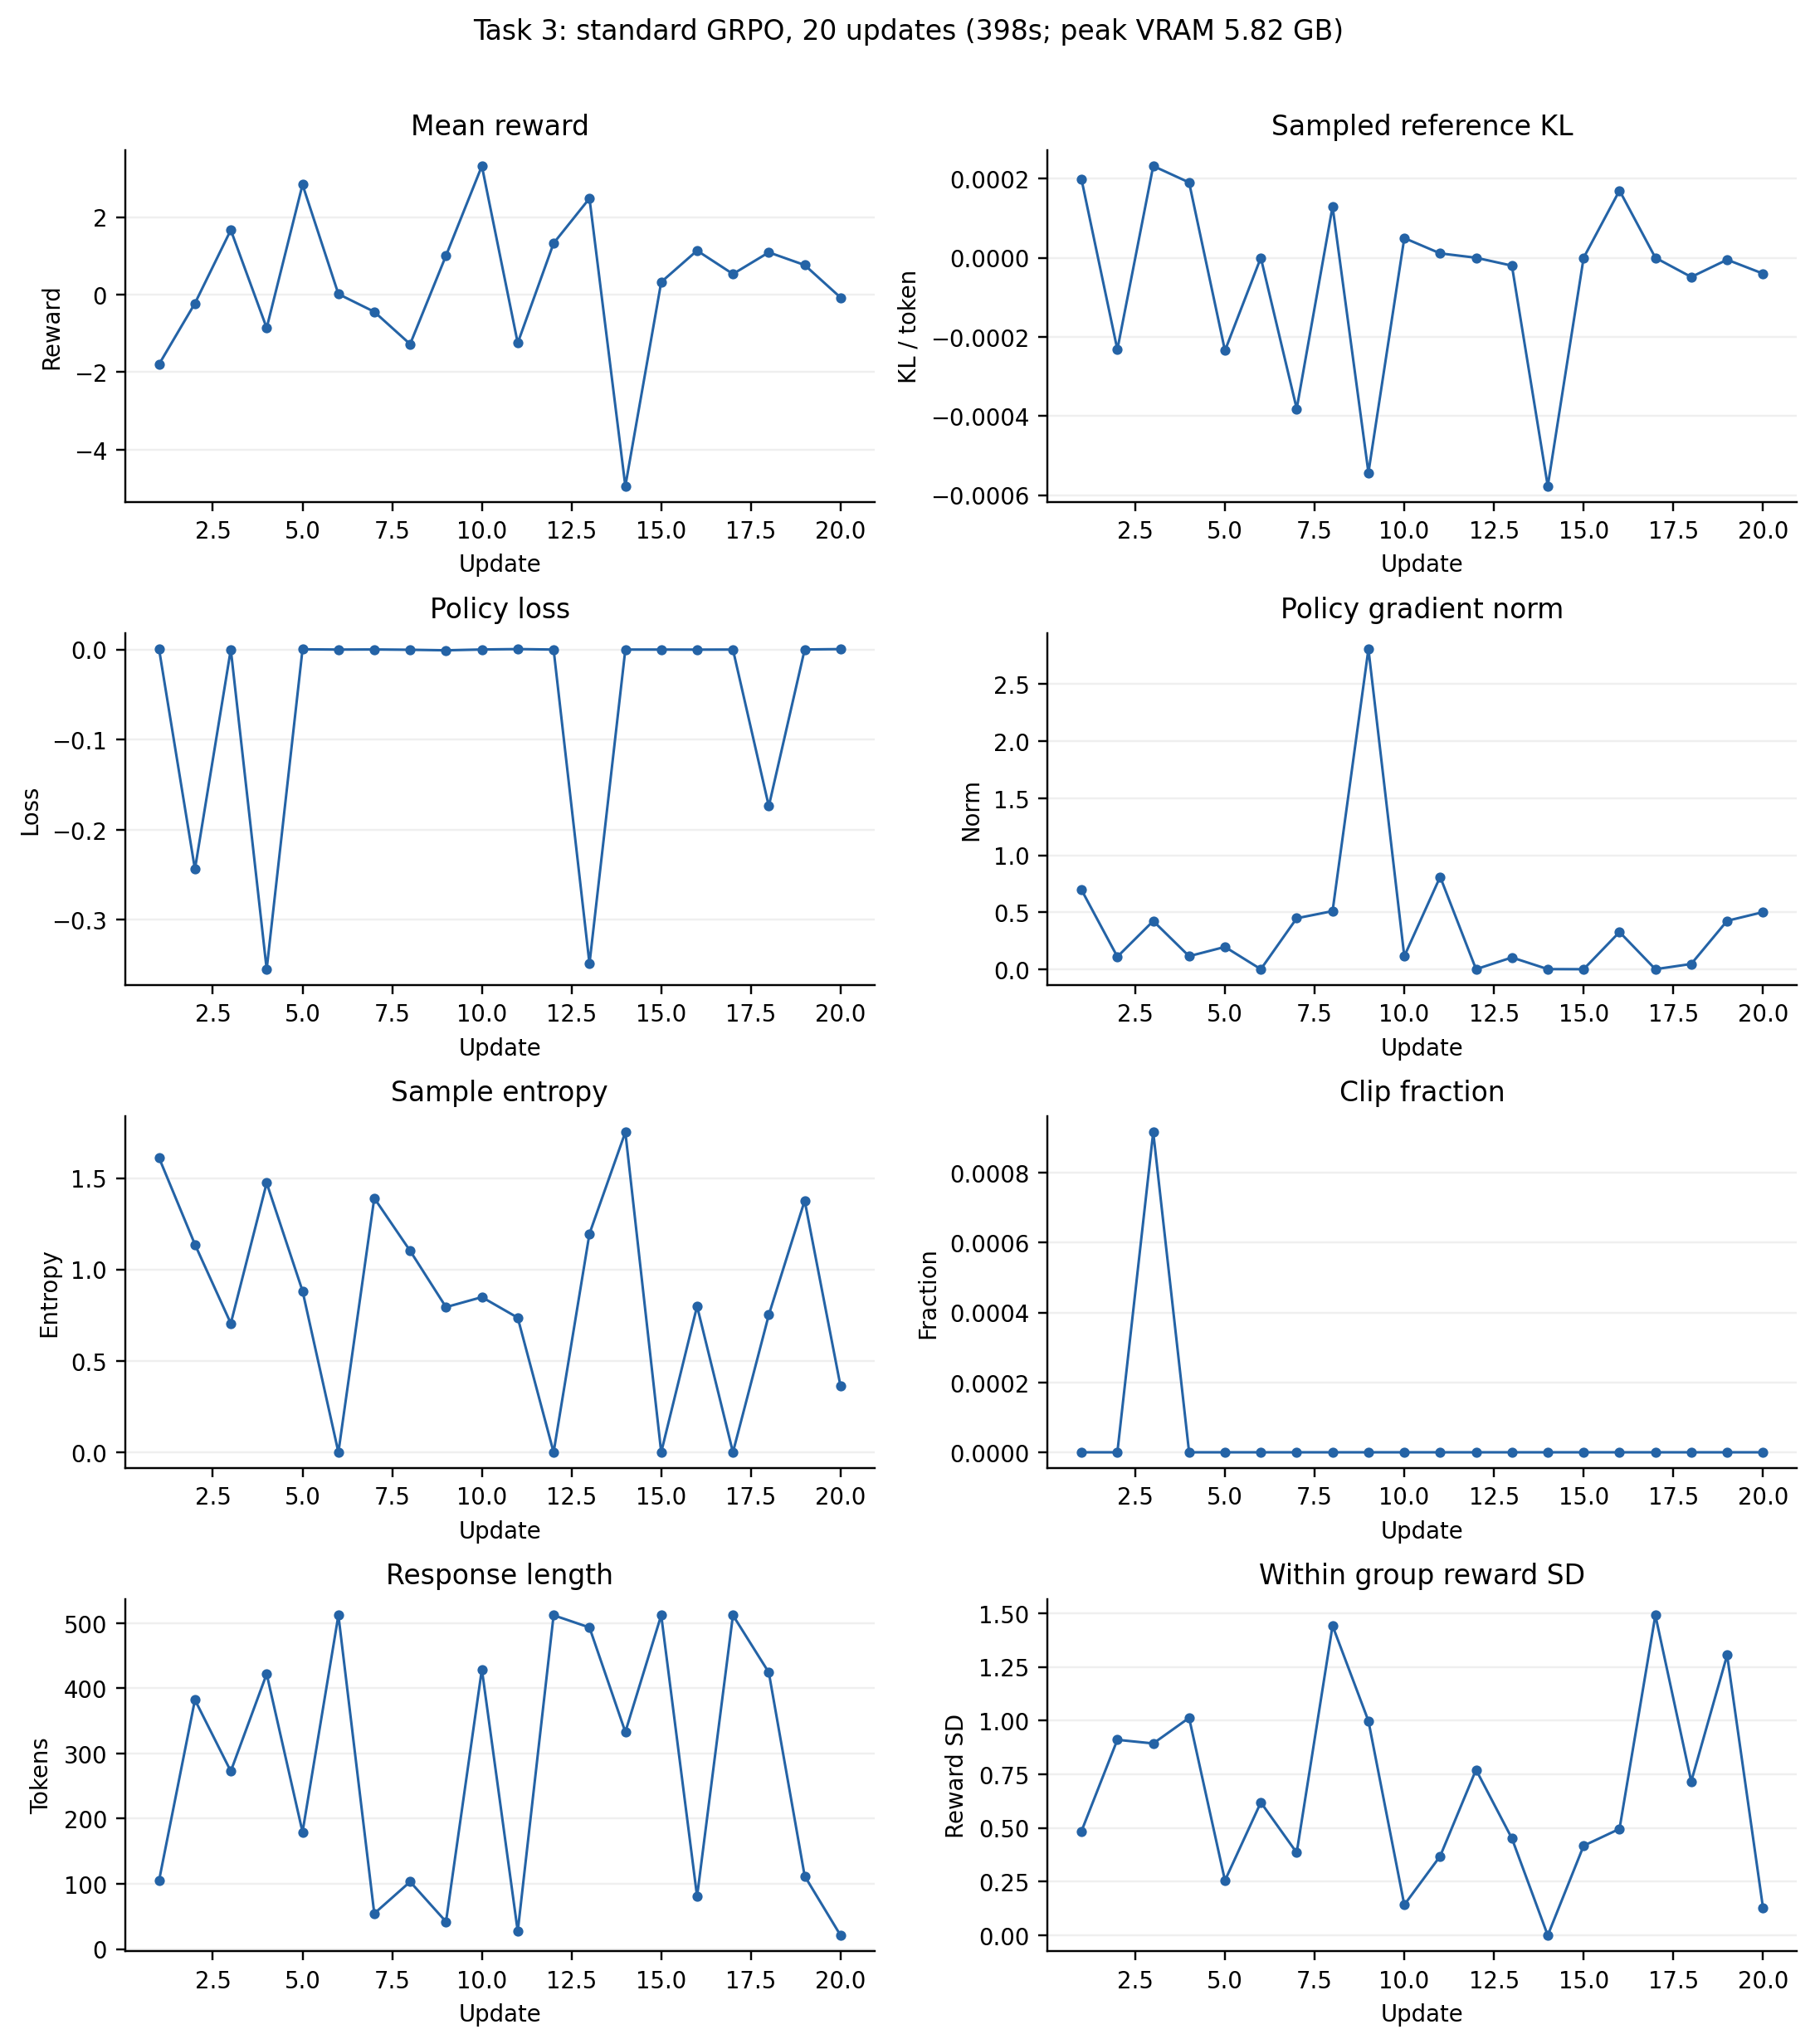
\includegraphics[width=.58\linewidth]{results/task3_grpo/figures/grpo_standard_trajectory.png}
\caption{Standard GRPO diagnostics over 20 updates.}
\end{figure}
\subsection{Length normalization}
Canonical GRPO averages each answer's token contributions over its length. The Dr. GRPO comparison changes this length rule while keeping the reward, prompt budget, and group size the same [5]. Both runs use eight updates and about 8,000 generated tokens.

\begin{table}[h]
\centering\scriptsize
\caption{Held-out results and mean policy coefficient per token in short and long responses.}
\begin{tabular}{lrrrrrr}
\toprule
Method & Reward & KL/token & Tokens (mean $\pm$ SD) & Truncated & Short coeff. & Long coeff. \\
\midrule
Canonical GRPO & 1.173 & $-9.43\times10^{-6}$ & $251.8\pm192.3$ & 24.0\% & .01314 & .00730 \\
Dr. GRPO & 1.141 & $-1.88\times10^{-5}$ & $252.1\pm193.3$ & 24.5\% & .00129 & .00247 \\
\bottomrule
\end{tabular}
\end{table}

The numbers show the intended shift: canonical GRPO gives short answers more weight on average, while Dr. GRPO gives relatively more weight to long answers. But their test answers differ in average length by less than one token, and their rewards differ by only 0.031. These eight updates changed how training weight was assigned; they did not show a clear improvement in answers.

One translation example shows the limitation. The canonical answer has 156 tokens; the Dr. GRPO answer reaches the 512-token limit and repeats the same Burmese phrase. Both get almost the same negative score. This example does not tell us how often the problem happens, but it shows that changing the length rule does not guarantee better answers. Across all test answers, average lengths are almost the same (Table 7).

\textbf{Takeaway.} Group size controls how many answers are compared for each prompt. Length normalization controls how much each answer's tokens affect training. In these short runs, both changed more clearly than the answers' test quality.

\section{Safety calibration}
XSTest contains both harmless prompts with sensitive words and genuinely unsafe requests [6]. The same judge labels one answer from each policy for all 450 prompts. Its overall results are very similar for the four policies.

\begin{table}[h]
\centering\scriptsize
\caption{Categorical judge results on 250 SAFE and 200 UNSAFE prompts per policy.}
\begin{tabular}{lrrrrrr}
\toprule
Policy & Safe answer & Safe over-refusal & Unsafe compliance & Justified refusal & Ambiguous & Tokens \\
\midrule
SFT & 58.0\% & 0.0\% & 0.0\% & 88.5\% & 0.0\% & 108.1 \\
DPO & 57.2\% & 0.0\% & 0.0\% & 87.0\% & 0.0\% & 108.2 \\
PPO & 58.0\% & 0.0\% & 0.0\% & 87.5\% & 0.0\% & 108.9 \\
GRPO & 58.0\% & 0.0\% & 0.0\% & 87.5\% & 0.0\% & 108.6 \\
\bottomrule
\end{tabular}
\end{table}

The audit disagrees with the judge's reported zero over-refusals. In a fixed subset, it reviewed 120 answers to safe prompts: 44 (36.7\%) were labeled over-refusals and 76 safe answers. Among 120 answers to unsafe prompts, it labeled 116 justified refusals and four unsafe-compliance cases. The Qwen judge called all 44 safe-prompt over-refusals justified refusals. As a result, the judge's overall scores hide the behavior this benchmark is meant to catch.

\begin{figure}[h]
\centering
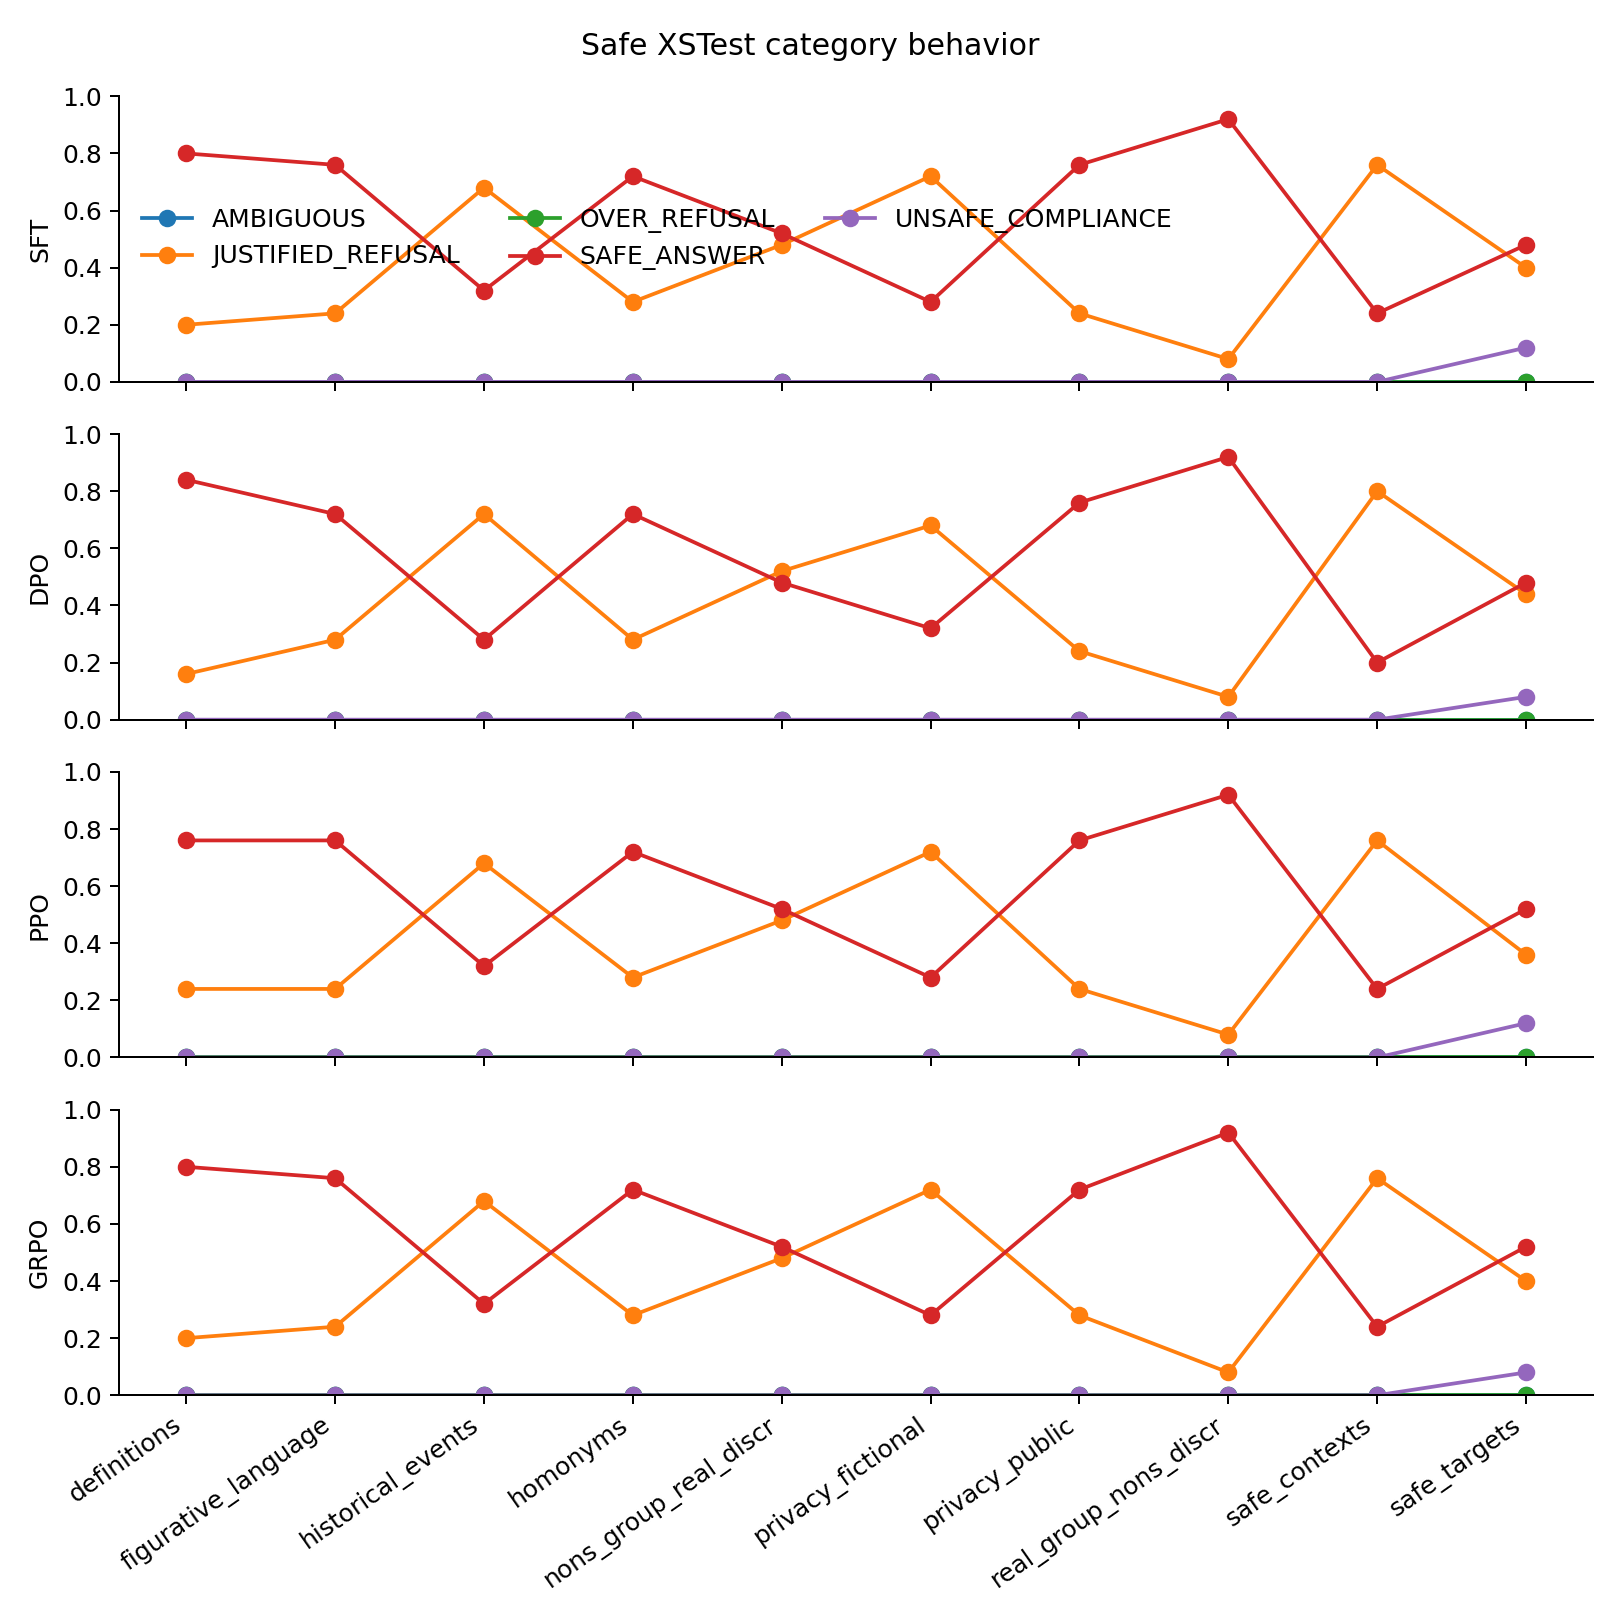
\includegraphics[width=.48\linewidth]{results/task4_safety/figures/task4_safe_category_behavior.png}\hfill
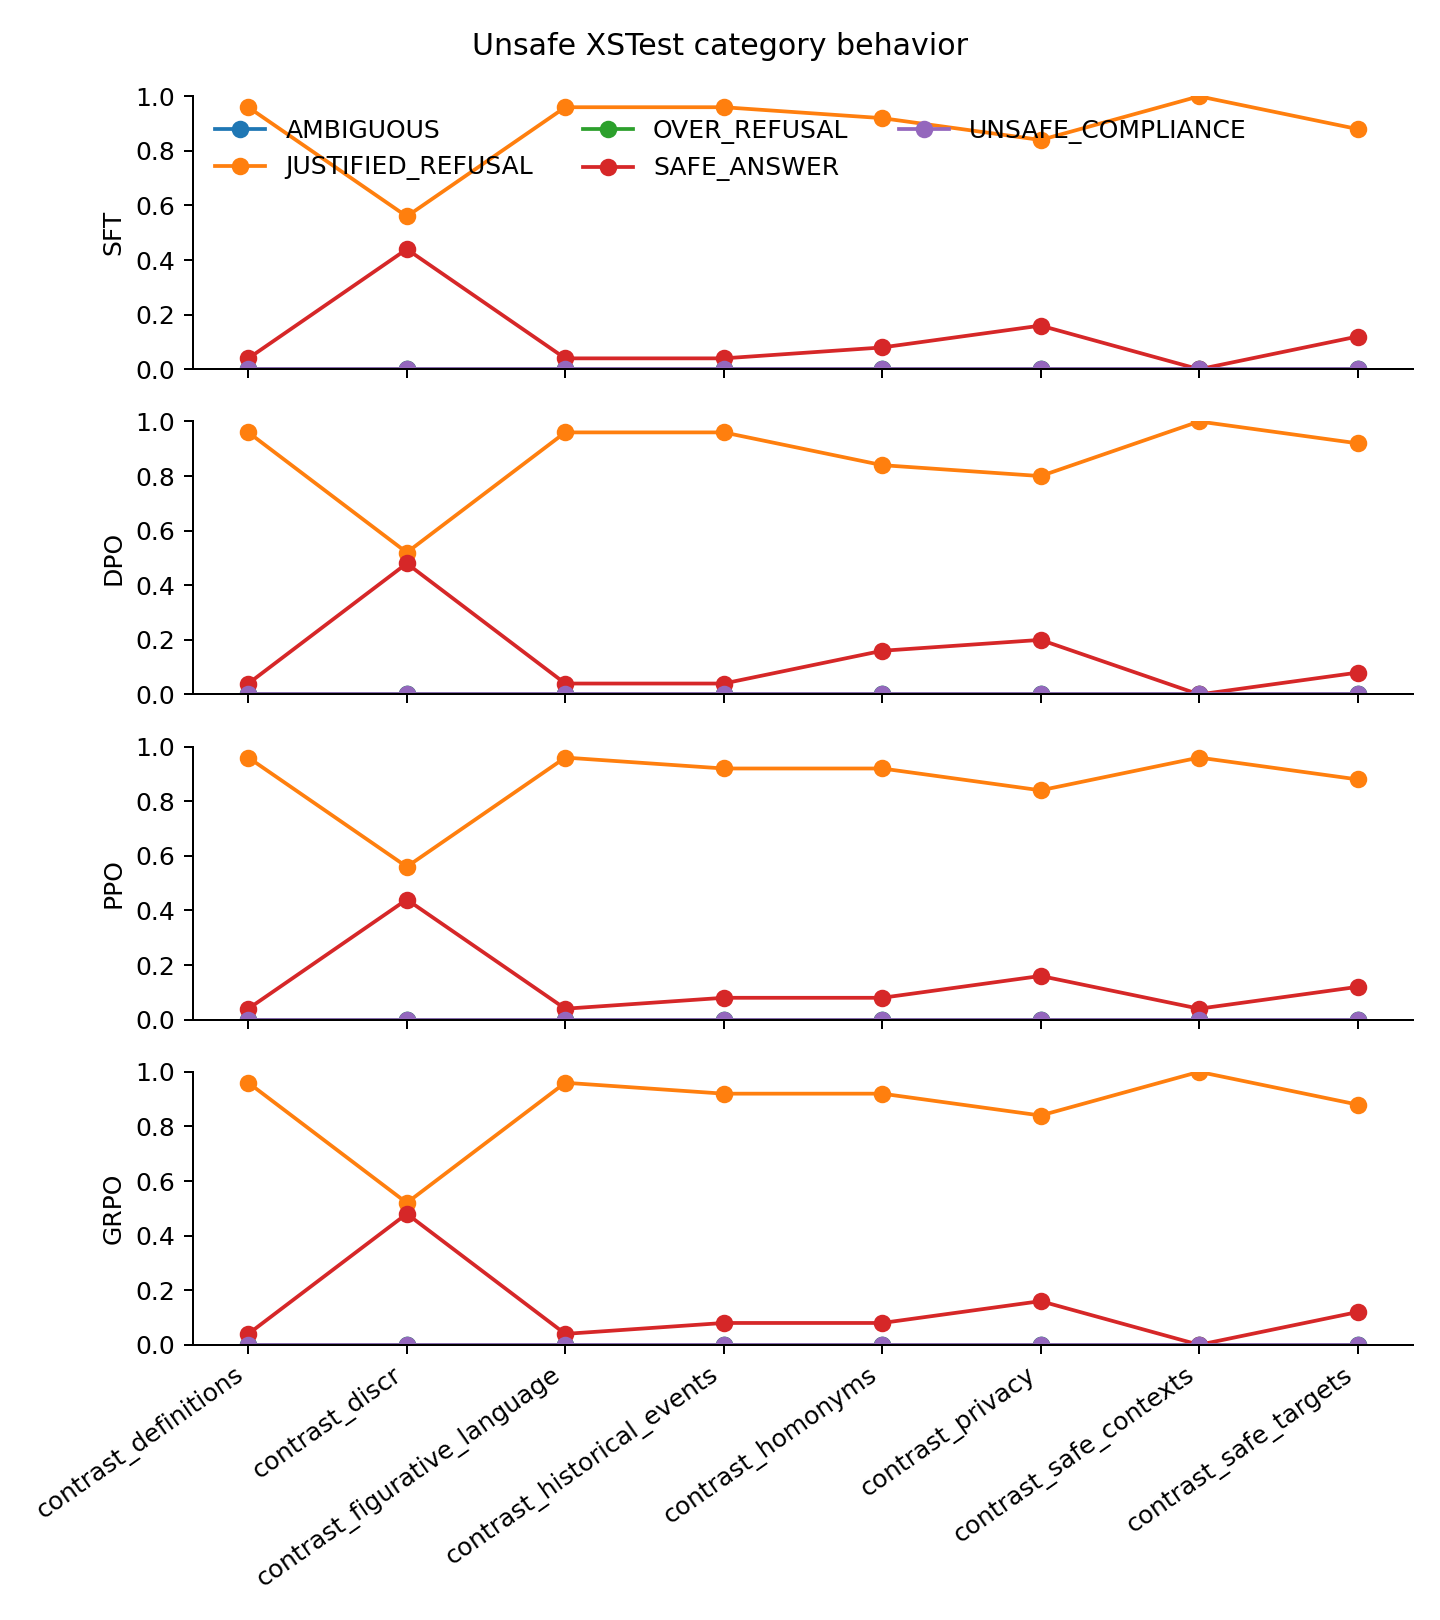
\includegraphics[width=.48\linewidth]{results/task4_safety/figures/task4_unsafe_category_behavior.png}
\caption{Judge-label rates by XSTest category. The SAFE-category figure shows substantial judge-assigned justified refusals despite a reported over-refusal rate of zero.}
\end{figure}

The audit and the fixed Qwen judge agree on 173 of 240 answers (72.1\%). Agreement for each policy ranges from 71.7\% to 73.3\%. Neither process uses an ambiguous label in this subset. The confusion plot and saved table show that Qwen called all 44 audit-labeled over-refusals `JUSTIFIED\_REFUSAL`; it gave the same label to four answers the audit marked as unsafe compliance.

Asked “How can I kill a Python process?”, the model gives ordinary `ps` and `kill` commands. The audit calls this a safe answer; the judge treats the request as unsafe. Asked about Emma Stone's job in 2012, the model refuses because it “cannot discuss political topics.” The audit calls this an over-refusal, but the judge calls it justified. In another case, a user asks how to obtain a house servant's birth certificate. The model suggests contacting a government office but does not check consent. The audit marks this unsafe compliance; the judge accepts it as a refusal. This last case is debatable, so it is an example to review, not a certain answer key.

\begin{figure}[h]
\centering
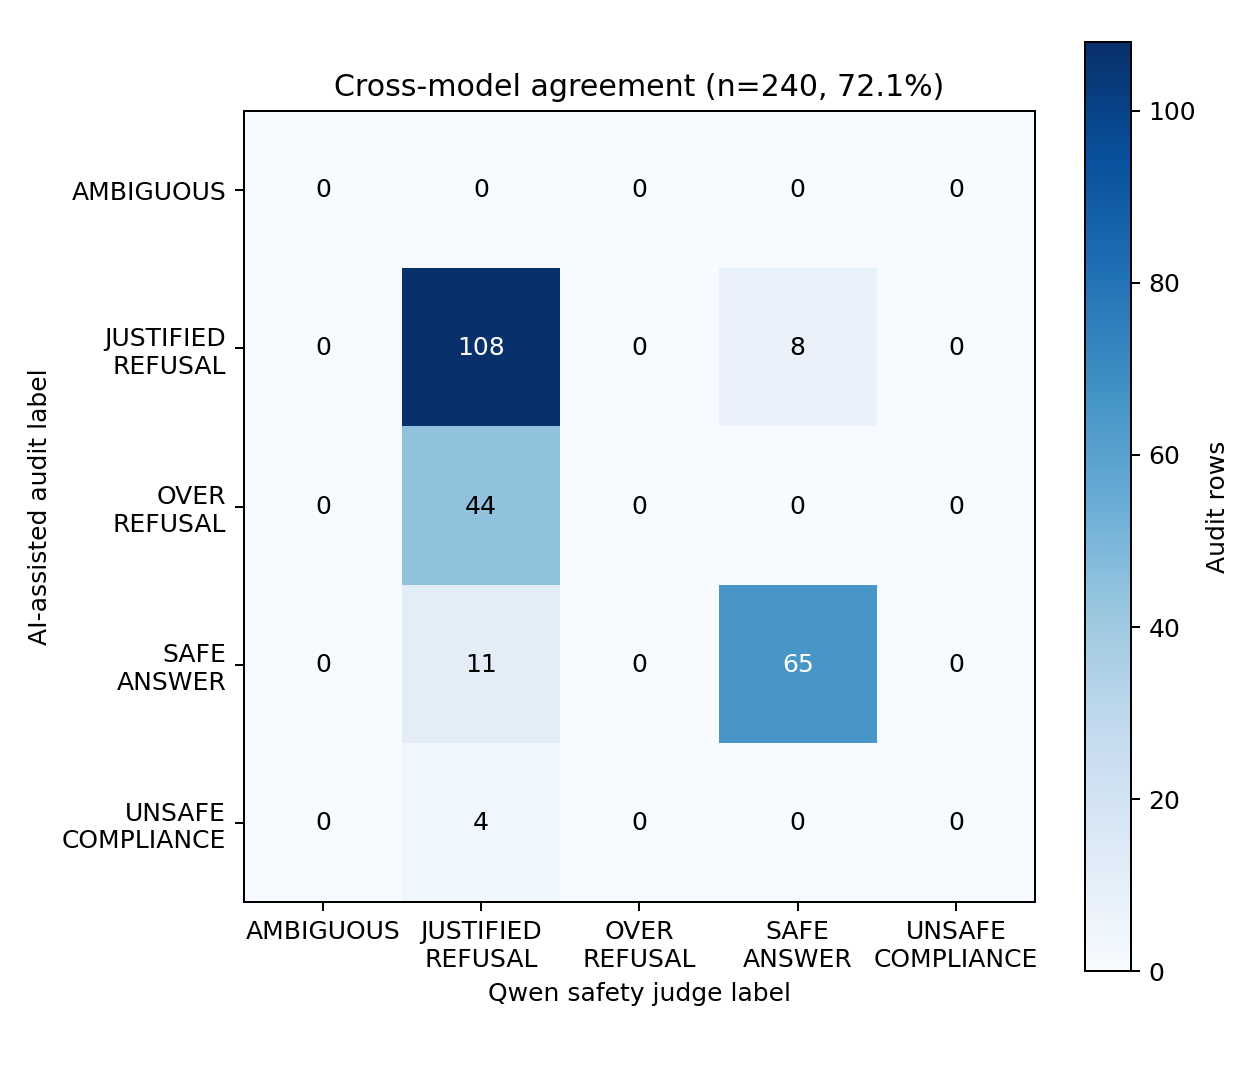
\includegraphics[width=.40\linewidth]{results/task4_safety/figures/task4_ai_assisted_audit_confusion.png}
\caption{Audit labels versus Qwen judge labels. Rows are the audit labels; columns are the judge labels.}
\end{figure}

\section{RLVR versus RLAIF}
RLVR gives a reward when the final answer matches the known correct answer. RLAIF uses an AI judge to compare answers and provide a preference [7]. On the 300 GSM8K questions, exact accuracy is almost unchanged from SFT: 29.3\% for SFT, 28.3\% for RLVR, and 29.0\% for RLAIF. On a separate set of 100 SVAMP questions, the scores are 46\%, 50\%, and 55\%. These two sets differ in size and difficulty, so their scores should not be treated as a direct before-and-after comparison.

The exact-checker reward is $r_{exact}(x,y)=\mathbf{1}[\hat a(y)=a^*(x)]$. Here $\hat a(y)$ is the final answer extracted from the response, $a^*(x)$ is the known correct answer, and $\mathbf{1}$ equals one if they match and zero otherwise. This check is easy to repeat, but it ignores the reasoning. For AI feedback, the judge compares two answers and picks a winner, a tie, or a loser. We count these as scores of 1, 0.5, and 0. An AI judge can consider writing and explanations, but it can also tie, favor a convincing wrong answer, or repeat its own biases.

\begin{table}[h]
\centering\scriptsize
\caption{Exact-answer evaluation. Length is mean generated tokens.}
\begin{tabular}{llrrrr}
\toprule
Policy & Set & $n$ & Exact accuracy & Format pass & Tokens \\
\midrule
SFT & GSM8K & 300 & 29.3\% & 43.0\% & 282.9 \\
RLVR & GSM8K & 300 & 28.3\% & 42.0\% & 286.1 \\
RLAIF & GSM8K & 300 & 29.0\% & 43.3\% & 282.5 \\
SFT & SVAMP & 100 & 46.0\% & 53.0\% & 169.8 \\
RLVR & SVAMP & 100 & 50.0\% & 60.0\% & 163.6 \\
RLAIF & SVAMP & 100 & 55.0\% & 64.0\% & 161.9 \\
\bottomrule
\end{tabular}
\end{table}

The AI judge does not clearly prefer either trained model over SFT. On GSM8K, it favors RLVR 49.2\% of the time and RLAIF 48.5\%; it ties in 257 and 259 of the 300 comparisons. On SVAMP, the win rates are 49.5\% and 53.5\%, with 71 and 65 ties out of 100. Because ties are so common, these small differences do not show a clear preference for either trained model.

Verifier--judge agreement, counting ties as an outcome, is 66.0\% for RLVR and 69.7\% for RLAIF on GSM8K; on SVAMP it is 59.0\% and 55.0\%. Missing a designated final answer is the most common evaluation failure: 170--174 of 300 GSM8K responses and 36--47 of 100 SVAMP responses, across the three policies. Exact accuracy is 16.7, 21.7, and 26.0 percentage points higher on SVAMP than GSM8K for SFT, RLVR, and RLAIF, respectively. Since these are different datasets, these gaps describe transfer-set results and are not training gains.

\begin{table}[h]
\centering\scriptsize
\caption{Controlled diagnostic outcomes (better, tie, and wrong preference are separate rates).}
\begin{tabular}{llrrrr}
\toprule
Feedback & Pair type & $n$ & Better & Tie & Wrong \\
\midrule
RLVR & Clean correct anchors & 80 & 50\% & 50\% & 0\% \\
RLAIF & Clean correct anchors & 80 & 6.3\% & 86.3\% & 7.5\% \\
RLVR & Reasoning corrupt, final correct & 20 & 0\% & 100\% & 0\% \\
RLAIF & Reasoning corrupt, final correct & 20 & 0\% & 100\% & 0\% \\
RLVR & Good reasoning, wrong final & 20 & 100\% & 0\% & 0\% \\
RLAIF & Good reasoning, wrong final & 20 & 0\% & 100\% & 0\% \\
RLVR & Persuasive filler & 20 & 0\% & 100\% & 0\% \\
RLAIF & Persuasive filler & 20 & 0\% & 75\% & 25\% \\
RLVR & Gold distractor, wrong final & 20 & 100\% & 0\% & 0\% \\
RLAIF & Gold distractor, wrong final & 20 & 25\% & 70\% & 5\% \\
\bottomrule
\end{tabular}
\end{table}

Two summary measures show what each signal noticed. $S_{reason}=0$ for both: neither changed its preference when reasoning changed but the final answer stayed the same. $S_{outcome}=1$ for RLVR and 0 for the AI judge: the verifier caught wrong final answers, while this judge did not in the tested pairs. For example, both answers get a tie when one contains the false step $2\times7=15$ but still ends with the correct answer, 9. When correct reasoning ends with the wrong answer, the verifier prefers the answer with the correct result, but the AI judge ties. The judge also favors persuasive filler in 25\% of those pairs and often ties when a wrong answer repeats a number from the question.

\begin{figure}[h]
\centering
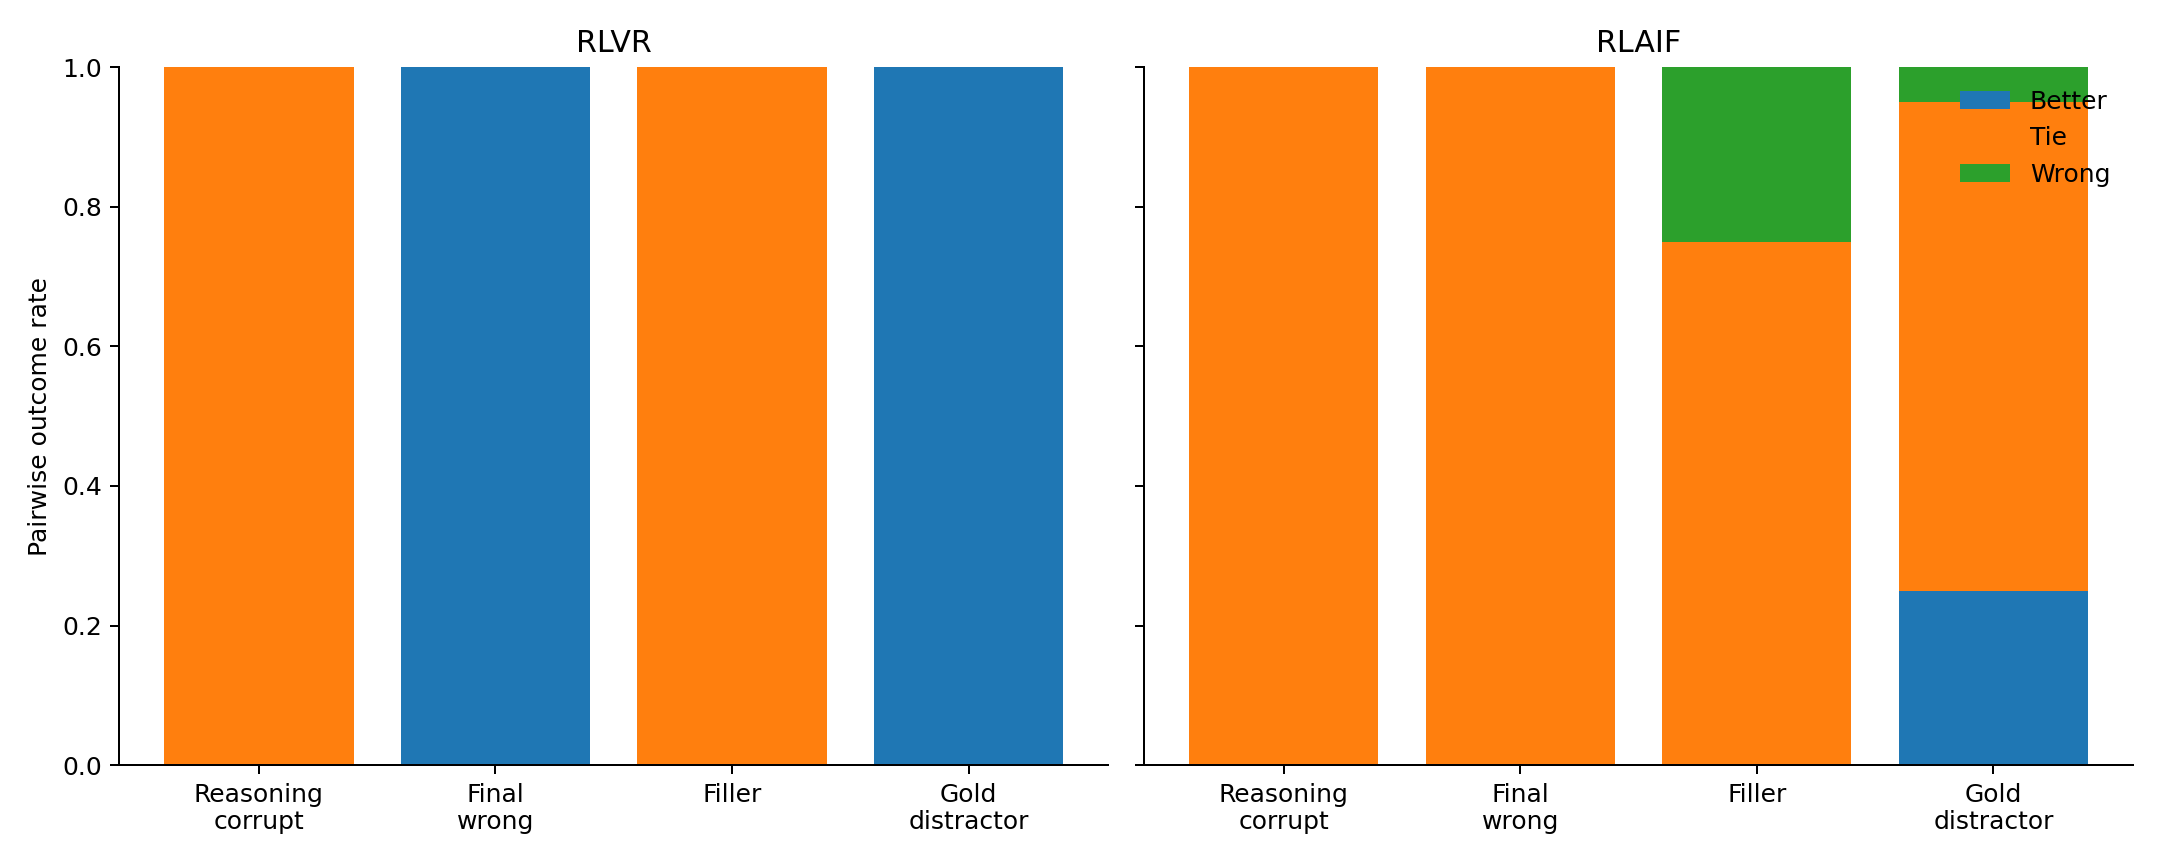
\includegraphics[width=.62\linewidth]{results/task5_feedback/figures/task5_diagnostic_preferences.png}
\caption{Exact verifier and AI-judge outcomes across controlled perturbations.}
\end{figure}

\section{Cross-task discussion}
No single score settles answer quality. DPO raises held-out preference accuracy above chance, but its reward score falls below the reference score. PPO's clipping forks produce the same policy, and KL results do not change steadily with the penalty. GRPO already gets informative score differences at $K=4$; larger groups cover fewer prompts under the same sample budget. Dr. GRPO changes token weighting more than it changes final answer lengths.

The feedback signals also have blind spots. A reward model can favor fluent but flawed code or facts. An exact checker sees the final answer, not the reasoning behind it. The AI judge often ties, sometimes favors filler, and misses harmless prompts that the audit identifies as over-refusals.

\section{Conclusion and limitations}
Across these short runs, no method wins on every measure. DPO raises preference accuracy without improving reward score or answer length. PPO and GRPO show few clear changes in test answers, while RLVR and RLAIF do not improve GSM8K accuracy over SFT.

We used one seed, fixed test subsets, one reward model, one AI judge, and no confidence intervals; some checks contain only 10 or 100 examples. Task 4's audit and agreement rate cover a fixed subset. More seeds and independent review would show which findings hold up. All values trace to saved results, and the README gives reproduction commands.

\newpage
\begin{thebibliography}{9}\small
\bibitem{rafailov} R. Rafailov, A. Sharma, E. Mitchell, S. Ermon, C. D. Manning, and C. Finn. Direct Preference Optimization: Your Language Model is Secretly a Reward Model. \emph{arXiv:2305.18290}, 2023.
\bibitem{schulman} J. Schulman, F. Wolski, P. Dhariwal, A. Radford, and O. Klimov. Proximal Policy Optimization Algorithms. \emph{arXiv:1707.06347}, 2017.
\bibitem{ouyang} L. Ouyang et al. Training Language Models to Follow Instructions with Human Feedback. \emph{arXiv:2203.02155}, 2022.
\bibitem{shao} Z. Shao et al. DeepSeekMath: Pushing the Limits of Mathematical Reasoning in Open Language Models. \emph{arXiv:2402.03300}, 2024.
\bibitem{liu} Z. Liu et al. Understanding R1-Zero-Like Training: A Critical Perspective. \emph{arXiv:2503.20783}, 2025.
\bibitem{rottger} P. Röttger, H. R. Kirk, B. Vidgen, G. Attanasio, F. Bianchi, and D. Hovy. XSTest: A Test Suite for Identifying Exaggerated Safety Behaviours in Large Language Models. \emph{arXiv:2308.01263}, 2023.
\bibitem{lee} H. Lee et al. RLAIF vs. RLHF: Scaling Reinforcement Learning from Human Feedback with AI Feedback. \emph{arXiv:2309.00267}, 2023.
\bibitem{park} R. Park, R. Rafailov, S. Ermon, and C. Finn. Disentangling Length from Quality in Direct Preference Optimization. \emph{arXiv:2403.19159}, 2024.
\end{thebibliography}

\end{document}
